\documentclass[11pt,a4paper]{article}

% Packages
\usepackage[utf8]{inputenc}
\usepackage[T1]{fontenc}
\usepackage{geometry}
\geometry{margin=1in, headheight=14pt}
\usepackage{graphicx}
\usepackage{amsmath,amssymb,amsthm}
\usepackage{algorithm}
\usepackage{algpseudocode}
\usepackage{booktabs}
\usepackage{hyperref}
\usepackage{xcolor}
\usepackage{listings}
\usepackage{caption}
\usepackage{subcaption}
\usepackage{tikz}
\usetikzlibrary{shapes,arrows.meta,positioning,fit,calc}
\usepackage{enumitem}
\usepackage{tcolorbox}
\usepackage{fancyhdr}
\usepackage{titlesec}

% Colors
\definecolor{codeblue}{HTML}{0366d6}
\definecolor{codegray}{HTML}{586069}
\definecolor{codebg}{HTML}{f6f8fa}
\definecolor{warnbg}{HTML}{fff3cd}
\definecolor{infobg}{HTML}{cce5ff}
\definecolor{dangerbg}{HTML}{f8d7da}

% Listings style
\lstdefinestyle{bashstyle}{
  language=bash,
  basicstyle=\ttfamily\small,
  backgroundcolor=\color{codebg},
  frame=single,
  rulecolor=\color{codegray},
  breaklines=true,
  columns=fullflexible,
  keepspaces=true,
  showstringspaces=false,
  commentstyle=\color{codegray}\itshape,
  keywordstyle=\color{codeblue}\bfseries,
}

\lstdefinestyle{pythonstyle}{
  language=Python,
  basicstyle=\ttfamily\small,
  backgroundcolor=\color{codebg},
  frame=single,
  rulecolor=\color{codegray},
  breaklines=true,
  columns=fullflexible,
  keepspaces=true,
  showstringspaces=false,
  commentstyle=\color{codegray}\itshape,
  keywordstyle=\color{codeblue}\bfseries,
  stringstyle=\color{red!60!black},
}

\lstdefinestyle{yamlstyle}{
  basicstyle=\ttfamily\small,
  backgroundcolor=\color{codebg},
  frame=single,
  rulecolor=\color{codegray},
  breaklines=true,
  columns=fullflexible,
  keepspaces=true,
  showstringspaces=false,
}

% tcolorbox environments
\newtcolorbox{warningbox}{
  colback=warnbg, colframe=orange!80!black,
  title={\textbf{Warning}}, fonttitle=\bfseries
}
\newtcolorbox{infobox}{
  colback=infobg, colframe=blue!60!black,
  title={\textbf{Note}}, fonttitle=\bfseries
}
\newtcolorbox{dangerbox}{
  colback=dangerbg, colframe=red!60!black,
  title={\textbf{Safety Critical}}, fonttitle=\bfseries
}

% Header
\pagestyle{fancy}
\fancyhf{}
\fancyhead[L]{\textit{Reach-Avoid Differential Game for UAVs}}
\fancyhead[R]{\textit{Project Documentation}}
\fancyfoot[C]{\thepage}

% Title formatting
\titleformat{\section}{\Large\bfseries}{}{0em}{}[\titlerule]
\titleformat{\subsection}{\large\bfseries}{}{0em}{}

% Theorems
\newtheorem{theorem}{Theorem}
\newtheorem{proposition}{Proposition}
\newtheorem{definition}{Definition}

\begin{document}

% Title page
\begin{titlepage}
\centering
\vspace*{3cm}
{\Huge\bfseries Reach-Avoid Differential Game\\[0.3cm] for UAV Interception\\[1cm]}
{\Large Implementation Documentation\\[0.5cm]}
\vspace{1.5cm}
{\large Based on the paper by Bui, Monckton, and Chen\\
\textit{``Reach-Avoid Differential Game with Reachability Analysis\\for UAVs --- A Decomposition Approach''}\\
(arXiv:2512.22793)}
\vspace{2cm}

\begin{tabular}{ll}
\textbf{Framework:} & Hamilton-Jacobi Reachability Analysis\\
\textbf{Solver:} & OptimizedDP-compatible API (hj\_reachability v0.7.0 backend)\\
\textbf{Simulation:} & Gazebo Harmonic + PX4 SITL\\
\textbf{Hardware:} & Crazyflie 2.1 + Crazyswarm2\\
\textbf{Middleware:} & ROS\,2 Humble\\
\textbf{Version:} & 0.3.0\\
\end{tabular}

\vfill
{\large \today}
\end{titlepage}

\tableofcontents
\newpage

%=============================================================================
\section{Project Overview}
%=============================================================================

This project implements a \textbf{3D reach-avoid differential game} between two unmanned aerial vehicles (UAVs). One drone, the \textbf{defender}, attempts to intercept a second drone, the \textbf{attacker}, before the attacker reaches a designated target region. The attacker simultaneously tries to navigate to its goal while avoiding both obstacles and the defender.

The core challenge is that computing optimal strategies for two drones in 3D space would require solving a Hamilton-Jacobi (HJ) partial differential equation on a \textbf{24-dimensional} joint state space (12 dimensions per quadrotor). This is computationally intractable. The paper introduces a \textbf{decomposition framework} that splits the problem into two solvable sub-games:

\begin{enumerate}
    \item \textbf{Horizontal sub-game (6D):} Models the x-y plane dynamics of both drones, including obstacles and the target region.
    \item \textbf{Vertical sub-game (3D):} Models the z-axis dynamics of both drones.
\end{enumerate}

Each sub-game is solved independently using HJ reachability analysis, and the solutions are recombined using a novel \textbf{reach-track control algorithm} that provides provable capture guarantees.

The implementation spans three layers:

\begin{itemize}
    \item \textbf{Offline computation:} Value functions are solved on a discretized grid using an OptimizedDP-compatible solver API (backed by \texttt{hj\_reachability} with JAX/GPU acceleration). These represent optimal strategies for all possible states.
    \item \textbf{Online control:} Real-time ROS\,2 controllers for both drones. The \textbf{defender} reads drone states, interpolates precomputed value functions, extracts optimal controls via gradient computation, and publishes velocity commands at 50\,Hz (with PID pursuit fallback outside the winning region). The \textbf{attacker} uses game-theoretic optimal control by default, extracting bang-bang velocity commands from the same value functions to optimally evade the defender while navigating toward the target.
    \item \textbf{Simulation \& hardware:} The game runs in Gazebo with PX4 autopilot for physics-based validation, as a lightweight kinematic simulation without PX4, or on real Crazyflie~2.1 drones with motion capture for state estimation.
\end{itemize}

\subsection{Key Results}

\begin{itemize}
    \item The decomposition reduces the problem from 24D (intractable) to a 6D + 3D pair (solvable in minutes to hours).
    \item Formal capture guarantees: if the initial state is in the defender's \textbf{winning region}, the defender is guaranteed to capture the attacker regardless of the attacker's strategy.
    \item The solution is \textbf{conservative}: the decomposition's winning region is a subset of the true optimal winning region, meaning the defender never falsely claims it can win.
\end{itemize}


%=============================================================================
\section{Mathematical Foundation}
%=============================================================================

\subsection{Dynamics Modeling}

Both drones are simplified from the full 12D quadrotor dynamics:

\begin{definition}[Defender --- Double Integrator]
The defender has inertia (cannot change velocity instantaneously):
\begin{equation}
\dot{x}_D = v_D, \qquad \dot{v}_D = K(u - v_D)
\label{eq:defender}
\end{equation}
where $u$ is the velocity command and $K = \text{diag}(k_x, k_y, k_z)$ are proportional gains. The state is 6D: position $(x_D, y_D, z_D)$ and velocity $(v_{D,x}, v_{D,y}, v_{D,z})$.
\end{definition}

\begin{definition}[Attacker --- Single Integrator]
The attacker has no inertia (controls velocity directly):
\begin{equation}
\dot{x}_A = d
\label{eq:attacker}
\end{equation}
where $d$ is the attacker's velocity command. The state is 3D: position $(x_A, y_A, z_A)$. This \textbf{overestimates} the attacker's capability, making the defender's strategy more conservative.
\end{definition}

\textbf{Speed constraints:}
\begin{align}
\|(u_x, u_y)\| &\leq U_D^h = 6~\text{m/s}, & \|(d_x, d_y)\| &\leq U_A^h = 3~\text{m/s} \\
|u_z| &\leq U_D^z = 4~\text{m/s}, & |d_z| &\leq U_A^z = 2~\text{m/s}
\end{align}

The defender is twice as fast as the attacker in all directions.

\subsection{Game Decomposition}

The capture condition is decomposed from a sphere into a \textbf{cylinder}:

\begin{itemize}
    \item \textbf{Original:} $\|p_A - p_D\|_2 \leq d_c$ \quad (spherical capture zone)
    \item \textbf{Decomposed:}
    \begin{align}
        \textbf{Horizontal:} \quad & \sqrt{(x_A - x_D)^2 + (y_A - y_D)^2} \leq d_h = 3~\text{m} \\
        \textbf{Vertical:} \quad & |z_A - z_D| \leq d_z = 1~\text{m}
    \end{align}
\end{itemize}

\textbf{Key assumption:} The target region $\mathcal{T}$ and obstacles depend only on horizontal $(x,y)$ coordinates, not altitude. This is practical for airspace corridor scenarios.

\subsection{Hamilton-Jacobi Reachability}

For each sub-game, we solve the HJ variational inequality backward in time:
\begin{equation}
\min\left\{\frac{\partial V}{\partial t} + H\left(x, \nabla_x V\right),\; V(x,t) - l(x)\right\} = 0
\label{eq:hji}
\end{equation}
where the Hamiltonian is:
\begin{equation}
H(x, p) = \max_u \min_d \; p \cdot f(x, u, d)
\end{equation}

The defender maximizes (tries to capture) and the attacker minimizes (tries to escape). The \textbf{zero level set} $\{x : V(x) \leq 0\}$ defines the winning region.

\subsection{Invariant Capture Sets}

Simply combining the two sub-game solutions does not guarantee simultaneous capture in both directions. The defender might overshoot vertically due to inertia while capturing horizontally. The solution uses \textbf{invariant capture sets}:

\begin{definition}[Invariant Capture Set $\mathcal{B}_z$]
$\mathcal{B}_z = \{x : V_{z,\infty}(x) \leq d_z\}$ where $V_{z,\infty}$ is the maximum distance value function. Once inside $\mathcal{B}_z$, the defender can keep $|z_D - z_A| \leq d_z$ \textbf{forever} using a tracking controller.
\end{definition}

\begin{definition}[Invariant Capture Set $\mathcal{B}_h$]
$\mathcal{B}_h = \{x : V_{h,T}(x) \leq d_h\}$ where $V_{h,T}$ is computed with $T = 2.5$\,s (does not converge as $T \to \infty$ due to the horizontal dynamics structure).
\end{definition}

These feed back into the reach-avoid computation: $\Phi_z$ uses $\mathcal{B}_z$ as its target set (Eq.~38 of the paper), and $\Phi_h$ uses the complement of $\mathcal{B}_h$ as part of its avoid set (Eq.~39).

\subsection{Computation Pipeline}

The correct computation order (matching the paper) is:

\begin{center}
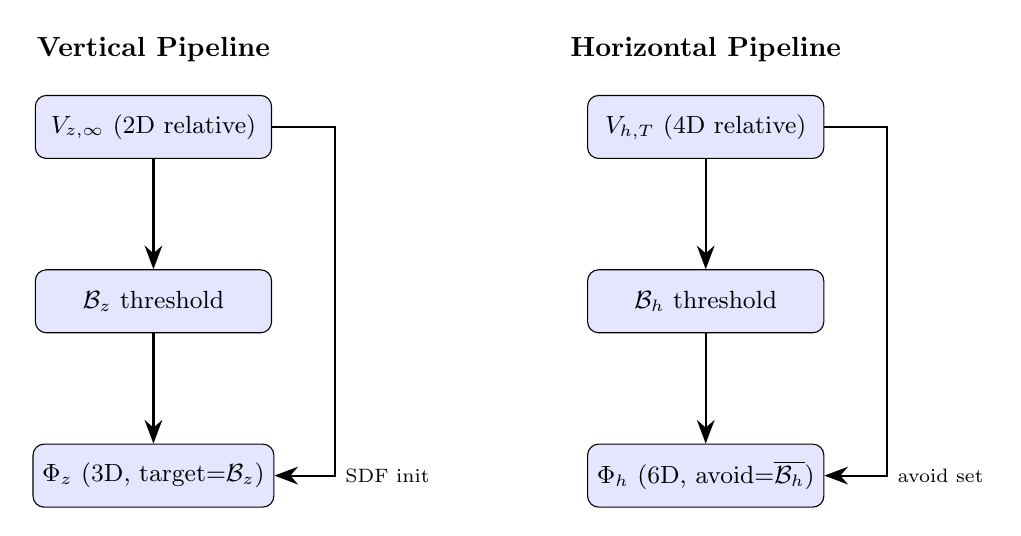
\begin{tikzpicture}[
    node distance=1.4cm,
    block/.style={rectangle, draw, rounded corners, fill=blue!10, minimum width=3cm, minimum height=0.8cm, align=center, font=\small},
    arrow/.style={-{Stealth[length=3mm]}, thick},
]
    % Vertical pipeline
    \node[block] (vzinf) {$V_{z,\infty}$ (2D relative)};
    \node[block, below=of vzinf] (bz) {$\mathcal{B}_z$ threshold};
    \node[block, below=of bz] (phiz) {$\Phi_z$ (3D, target=$\mathcal{B}_z$)};

    \draw[arrow] (vzinf) -- (bz);
    \draw[arrow] (bz) -- (phiz);
    \draw[arrow] (vzinf.east) -- ++(0.8,0) |- (phiz.east) node[midway, right, font=\scriptsize] {SDF init};

    % Horizontal pipeline
    \node[block, right=4cm of vzinf] (vht) {$V_{h,T}$ (4D relative)};
    \node[block, below=of vht] (bh) {$\mathcal{B}_h$ threshold};
    \node[block, below=of bh] (phih) {$\Phi_h$ (6D, avoid=$\overline{\mathcal{B}_h}$)};

    \draw[arrow] (vht) -- (bh);
    \draw[arrow] (bh) -- (phih);
    \draw[arrow] (vht.east) -- ++(0.8,0) |- (phih.east) node[midway, right, font=\scriptsize] {avoid set};

    % Labels
    \node[above=0.3cm of vzinf, font=\bfseries] {Vertical Pipeline};
    \node[above=0.3cm of vht, font=\bfseries] {Horizontal Pipeline};
\end{tikzpicture}
\end{center}

\subsection{Capture Guarantee Analysis}

\begin{theorem}[Defender Wins]
The defender is guaranteed to capture the attacker if all of the following hold:
\begin{enumerate}
    \item $x^z \in \mathcal{W}_{D,z}$ --- vertical state is in defender's vertical winning region
    \item $T_\text{goal} > T_\text{capture}$ --- defender captures vertically before attacker reaches goal
    \item $x^h \in \mathcal{W}_{D,h}$ --- horizontal state is in defender's horizontal winning region
\end{enumerate}
\end{theorem}

Where $T_\text{goal}$ is the earliest time the attacker can reach its target (from $\Phi_{A,\text{reach}}$) and $T_\text{capture}$ is the earliest time the defender achieves vertical capture (from $\Phi_z$ time slices).


%=============================================================================
\section{Implementation Architecture}
%=============================================================================

\subsection{Repository Structure}

\begin{lstlisting}[style=bashstyle, title=\textbf{Top-Level Directory Layout}]
/workspace/
  config/
    game_params.yaml        # Game parameters and grid presets
  data/
    value_functions/        # Precomputed .npz value function files
    plots/paper_figures/    # Generated paper figures
    simulations/            # Simulation trajectory outputs
  reach_avoid_game/         # Core Python package (offline computation)
    src/reach_avoid_game/
      config.py             # GameConfig dataclass
      dynamics/             # HJ dynamics classes (dual API)
      solvers/              # HJ solvers and utilities
      odp/                  # OptimizedDP-compatible API layer
        grid.py             # Grid class (NumPy, matches ODP API)
        solver.py           # HJSolver wrapper + computeSpatDerivArray
        shapes.py           # Shape functions for initial values
      visualization/        # Plotting functions
    scripts/                # CLI entry points
    tests/                  # Pytest test suite (60 tests)
  tests/
    integration/
      test_kinematic_game.py  # Standalone end-to-end simulation
  reach_avoid_ws/           # ROS 2 workspace (online control)
    src/
      reach_avoid_bringup/  # Launch files and parameters
      reach_avoid_sim/      # Gazebo adapters, PX4 bridge
      reach_avoid_controller/ # Defender reach-track controller
      attacker_controller/  # Attacker control modes
      reach_avoid_viz/      # RViz MarkerArray visualization
      reach_avoid_hw/       # Crazyflie hardware interface
\end{lstlisting}

\subsection{Offline Computation Package: \texttt{reach\_avoid\_game}}

\subsubsection{OptimizedDP-Compatible Solver API (\texttt{odp/})}

A custom OptimizedDP-compatible package provides the paper's solver API without requiring HeteroCL (which is only available for Python~3.8 via conda). The package includes:

\begin{itemize}
    \item \texttt{grid.py}: \texttt{Grid(minBounds, maxBounds, dims, pts\_each\_dim, periodicDims)} --- same API as \texttt{odp.Grid.GridProcessing.Grid} from the SFU-MARS OptimizedDP repository.
    \item \texttt{solver.py}: \texttt{HJSolver(dynamics, grid, values, tau, compMethod)} --- OptimizedDP-compatible entry point that delegates to \texttt{hj\_reachability}'s proven Lax-Friedrichs solver internally. Also provides \texttt{computeSpatDerivArray(grid, V, dim)} for spatial derivative extraction.
    \item \texttt{shapes.py}: \texttt{CylinderShape}, \texttt{ShapeRectangle} for constructing initial value function SDFs.
\end{itemize}

The \texttt{HJSolver} translates OptimizedDP's \texttt{compMethod} dictionary to \texttt{hj\_reachability} solver settings:

\begin{table}[h]
\centering
\small
\caption{Mapping between OptimizedDP and hj\_reachability solver modes.}
\begin{tabular}{lp{6cm}}
\toprule
\textbf{OptimizedDP \texttt{compMethod}} & \textbf{hj\_reachability equivalent} \\
\midrule
\texttt{"TargetSetMode": "minVWithV0"} & Backward Reachable Tube ($V = \min(V, V_0)$) \\
\texttt{"TargetSetMode": "maxVWithV0"} & Max-over-time ($V = \max(V, V_0)$) \\
\texttt{"ObstacleSetMode": "maxVWithObstacle"} & Reach-avoid with obstacle constraint \\
\texttt{"TargetSetMode": "none"} & Pure backward reachable set \\
\bottomrule
\end{tabular}
\end{table}

\subsubsection{Dynamics Classes}

Each dynamics class inherits from \texttt{hj.ControlAndDisturbanceAffineDynamics} (for the HJ solver) and additionally provides OptimizedDP-style pure-Python methods for online control extraction. The class implements three hj\_reachability methods:

\begin{table}[h]
\centering
\caption{Dynamics classes and their state spaces.}
\begin{tabular}{lccl}
\toprule
\textbf{Class} & \textbf{Dim} & \textbf{State} & \textbf{File} \\
\midrule
\texttt{VerticalGameDynamics} & 3D & $(z_D, v_{D,z}, z_A)$ & \texttt{vertical\_game.py} \\
\texttt{VerticalRelativeDynamics} & 2D & $(z_\text{rel}, v_{D,z})$ & \texttt{vertical\_relative.py} \\
\texttt{HorizontalGameDynamics} & 6D & $(x_D, y_D, v_{D,x}, v_{D,y}, x_A, y_A)$ & \texttt{horizontal\_game.py} \\
\texttt{HorizontalRelativeDynamics} & 4D & $(x_\text{rel}, y_\text{rel}, v_{D,x}, v_{D,y})$ & \texttt{horizontal\_relative.py} \\
\texttt{HorizontalGameTrackingDynamics} & 6D & same as above & \texttt{horizontal\_game.py} \\
\texttt{AttackerReachingDynamics} & 2D & $(x_A, y_A)$ & \texttt{attacker\_reaching.py} \\
\bottomrule
\end{tabular}
\end{table}

Each class provides the \textbf{hj\_reachability interface} (for the solver):
\begin{itemize}
    \item \texttt{open\_loop\_dynamics(state, time)} --- drift dynamics $f(x)$ when $u = 0$, $d = 0$
    \item \texttt{control\_jacobian(state, time)} --- matrix $G_u$ mapping control to state derivatives
    \item \texttt{disturbance\_jacobian(state, time)} --- matrix $G_d$ mapping disturbance to state derivatives
\end{itemize}

Key classes also provide the \textbf{OptimizedDP-compatible NumPy methods} (for online control extraction):
\begin{itemize}
    \item \texttt{opt\_ctrl\_numpy(state, spat\_deriv)} --- optimal control from value function gradient
    \item \texttt{opt\_dstb\_numpy(state, spat\_deriv)} --- optimal disturbance from gradient
    \item \texttt{dynamics\_numpy(state, u, d)} --- state derivatives given control and disturbance
\end{itemize}

The \texttt{HorizontalGameTrackingDynamics} class is identical to \texttt{HorizontalGameDynamics} except with \textbf{swapped optimization}: \texttt{control\_mode="min"} (defender minimizes distance) and \texttt{disturbance\_mode="max"} (attacker maximizes distance). This is used for computing the maximum distance value function $V_{h,T}$ in 6D coordinates with obstacle penalties.

\subsubsection{Solver Functions}

All solvers are in the \texttt{solvers/} subdirectory:

\begin{table}[h]
\centering
\caption{Value functions computed by each solver function.}
\begin{tabular}{llcp{5.5cm}}
\toprule
\textbf{Function} & \textbf{Output} & \textbf{Grid} & \textbf{Description} \\
\midrule
\texttt{solve\_vertical\_max\_distance} & $V_{z,\infty}$ & 2D & Max distance tracking (converged) \\
\texttt{compute\_invariant\_set\_Bz} & $\mathcal{B}_z$ & 2D & Threshold $V_{z,\infty} \leq d_z$ \\
\texttt{solve\_vertical\_reach\_avoid} & $\Phi_z$ & 3D & Vertical reach-avoid with $\mathcal{B}_z$ target \\
\texttt{solve\_horizontal\_max\_distance} & $V_{h,T}$ & 4D & Max distance tracking ($T=2.5$\,s) \\
\texttt{compute\_invariant\_set\_Bh} & $\mathcal{B}_h$ & 4D & Threshold $V_{h,T} \leq d_h$ \\
\texttt{solve\_attacker\_reaching} & $\Phi_{A,\text{reach}}$ & 2D & Attacker time-to-goal \\
\texttt{solve\_horizontal\_reach\_avoid} & $\Phi_h$ & 6D & Horizontal reach-avoid with $\overline{\mathcal{B}_h}$ avoid \\
\texttt{solve\_horizontal\_max\_distance\_6d} & $V_{h,T}^{6D}$ & 6D & 6D extension with obstacles \\
\bottomrule
\end{tabular}
\end{table}

\subsubsection{Control Extraction}

Optimal controls are extracted from value function gradients using central finite differences:

\begin{equation}
\nabla V(x) \approx \left[\frac{V(x + h\,e_i) - V(x - h\,e_i)}{2h}\right]_{i=1}^n
\end{equation}

The defender's optimal control (maximizing the value function):
\begin{equation}
u_z^* = U_{D,z} \cdot \text{sign}\!\left(\frac{\partial V}{\partial v_{D,z}} \cdot k_z\right)
\end{equation}

The attacker's optimal disturbance (minimizing the value function):
\begin{equation}
d_z^* = -U_{A,z} \cdot \text{sign}\!\left(\frac{\partial V}{\partial z_A}\right)
\end{equation}

Value function interpolation uses \texttt{scipy.interpolate.RegularGridInterpolator} with linear interpolation and appropriate boundary handling (\texttt{fill\_value} set to large positive values for out-of-domain queries).

\subsubsection{Winning Conditions}

The \texttt{winning\_conditions.py} module implements:

\begin{itemize}
    \item \texttt{compute\_T\_goal}: Estimates earliest time the attacker reaches its target from $\Phi_{A,\text{reach}}$.
    \item \texttt{compute\_T\_capture}: Estimates vertical capture time from $\Phi_z$ magnitude.
    \item \texttt{compute\_T\_capture\_from\_slices}: The paper-accurate method --- iterates through saved $\Phi_z$ time slices and finds the first time at which $\Phi_z(x, t) \leq 0$.
    \item \texttt{check\_defender\_wins}: Combined check of all winning conditions.
    \item \texttt{get\_winning\_regions}: Extracts $\mathcal{W}_D$ and $\mathcal{W}_A$ masks from a value function.
\end{itemize}

\subsubsection{Value Function I/O}

All value functions are stored as NumPy \texttt{.npz} files with a standardized format:

\begin{lstlisting}[style=pythonstyle]
@dataclass
class ValueFunctionData:
    values: np.ndarray       # The value function array
    grid_min: np.ndarray     # Grid lower bounds
    grid_max: np.ndarray     # Grid upper bounds
    grid_shape: tuple        # Grid dimensions
    params: dict             # Game parameters used
    description: str         # Human-readable description
\end{lstlisting}

Time slices (for $T_\text{capture}$ extraction) are stored separately as \texttt{phi\_z\_time\_slices.npz} containing the full time evolution of $\Phi_z$.

\subsection{Online Control: ROS\,2 Workspace}

\subsubsection{Package Overview}

\begin{table}[h]
\centering
\caption{ROS\,2 packages and their roles.}
\begin{tabular}{lp{8cm}}
\toprule
\textbf{Package} & \textbf{Purpose} \\
\midrule
\texttt{reach\_avoid\_bringup} & Launch files, configuration YAML, dependency management \\
\texttt{reach\_avoid\_sim} & PX4 adapter (MAVLink $\leftrightarrow$ ROS\,2), ground truth relay from Gazebo \\
\texttt{reach\_avoid\_controller} & Defender controller implementing Algorithms 1 \& 2 with value function lookup \\
\texttt{attacker\_controller} & Attacker with modes: optimal (default, HJ bang-bang control), scripted waypoints, keyboard teleop, switchable \\
\texttt{reach\_avoid\_viz} & MarkerArray publisher for obstacles, target, capture zones in RViz \\
\texttt{reach\_avoid\_hw} & Crazyswarm2 adapter for Crazyflie drones, safety monitor \\
\bottomrule
\end{tabular}
\end{table}

\subsubsection{Defender Controller Node}

The \texttt{DefenderControllerNode} runs at 50\,Hz and implements the two-algorithm reach-track controller:

\begin{algorithm}[H]
\caption{Vertical Reach-Track (Algorithm 1) --- with winning region guard}
\begin{algorithmic}[1]
\State \textbf{Input:} Vertical state $(z_D, v_{D,z}, z_A)$, value functions $\Phi_z$, $V_{z,\infty}$, $\mathcal{B}_z$
\State Compute $z_\text{rel} \gets z_D - z_A$
\State $\textit{in\_winning} \gets \Phi_z(z_D, v_{D,z}, z_A) \leq 0$ \Comment{Check defender's winning region}
\State Look up $\mathcal{B}_z(z_\text{rel}, v_{D,z})$
\If{NOT in $\mathcal{B}_z$}
    \If{$\textit{in\_winning}$}
        \State $u_z \gets$ optimal reaching control from $\nabla\Phi_z$ \Comment{Mode: REACHING}
    \Else
        \State $u_z \gets \text{PID}(z_A - z_D)$ \Comment{Mode: PID\_PURSUIT}
    \EndIf
\ElsIf{deep inside $\mathcal{B}_z$}
    \State $u_z \gets \text{PID}(z_A - z_D)$ \Comment{Mode: PID\_DEEP}
\Else
    \State $u_z \gets$ optimal tracking control from $\nabla V_{z,\infty}$ \Comment{Mode: TRACKING}
\EndIf
\State \Return $u_z$
\end{algorithmic}
\end{algorithm}

\begin{infobox}
The \textbf{winning region guard} ($\Phi \leq 0$ check) is critical for robustness. The paper's optimal HJ controls are only valid inside the winning region. On coarse grids (e.g., the \texttt{dev} preset with a $9 \times 7 \times 5 \times 5 \times 9 \times 7$ 6D grid), $\Phi_h > 0$ everywhere, meaning value function gradients point in arbitrary directions. PID pursuit provides a reliable fallback that always drives the defender toward the attacker.
\end{infobox}

\begin{algorithm}[H]
\caption{Horizontal Reach-Track-Avoid (Algorithm 2) --- with winning region guard}
\begin{algorithmic}[1]
\State \textbf{Input:} Horizontal state $(x_D, y_D, v_{D,x}, v_{D,y}, x_A, y_A)$, value functions $\Phi_h$, $V_{h,T}$, $\mathcal{B}_h$
\State $\textit{in\_winning} \gets \Phi_h(x_D, y_D, v_{D,x}, v_{D,y}, x_A, y_A) \leq 0$ \Comment{Check winning region}
\State Compute relative state $(x_\text{rel}, y_\text{rel}, v_{D,x}, v_{D,y})$
\State Look up $\mathcal{B}_h(x_\text{rel}, y_\text{rel}, v_{D,x}, v_{D,y})$
\If{NOT in $\mathcal{B}_h$}
    \If{$\textit{in\_winning}$}
        \State $(u_x, u_y) \gets$ optimal reaching control from $\nabla\Phi_h$ \Comment{Mode: REACHING}
    \Else
        \State $(u_x, u_y) \gets \text{PID}(x_A - x_D, y_A - y_D)$ \Comment{Mode: PID\_PURSUIT}
    \EndIf
\ElsIf{deep inside $\mathcal{B}_h$}
    \State $(u_x, u_y) \gets \text{PID}(x_A - x_D, y_A - y_D)$ \Comment{Mode: PID\_DEEP}
\Else
    \State $(u_x, u_y) \gets$ optimal tracking control from $\nabla V_{h,T}$ \Comment{Mode: TRACKING}
\EndIf
\State \Return $(u_x, u_y)$
\end{algorithmic}
\end{algorithm}

\subsubsection{Attacker Controller Node}

The \texttt{AttackerControllerNode} runs at 20\,Hz and supports multiple control modes. The default mode is \texttt{optimal}, which implements game-theoretic bang-bang control using Hamilton-Jacobi value function gradients.

\paragraph{Optimal Control Mode.}
The attacker acts as the \textbf{disturbance} player in the HJ game formulation, minimizing the value function to optimally evade the defender while heading toward the target. The control law is bang-bang (always at maximum speed):

\begin{align}
d_x^* &= -U_A^h \cdot \text{sign}\!\left(\frac{\partial \Phi_h}{\partial x_A}\right), &
d_y^* &= -U_A^h \cdot \text{sign}\!\left(\frac{\partial \Phi_h}{\partial y_A}\right) \label{eq:attacker-horiz}\\[4pt]
d_z^* &= -U_A^z \cdot \text{sign}\!\left(\frac{\partial \Phi_z}{\partial z_A}\right) \label{eq:attacker-vert}
\end{align}

where:
\begin{itemize}[noitemsep]
    \item $\Phi_h$ is the 6D horizontal game value function with state $[x_D, y_D, v_{D,x}, v_{D,y}, x_A, y_A]$
    \item $\Phi_z$ is the 3D vertical game value function with state $[z_D, v_{D,z}, z_A]$
    \item $U_A^h = 3.0$\,m/s (max horizontal speed), $U_A^z = 2.0$\,m/s (max vertical speed)
    \item Gradients at indices 4,\,5 (for $x_A, y_A$) and index 2 (for $z_A$) respectively
\end{itemize}

The negative sign reflects the attacker's role as the \textbf{minimizer} in the game (opposite to the defender, who maximizes). This ensures the attacker moves in the direction that most decreases the value function, corresponding to the worst-case disturbance from the defender's perspective.

\paragraph{Fallback Behavior.}
If the value function gradient is near-zero (e.g., at grid boundaries) or the defender's state is not yet available, the attacker falls back to \textbf{simple goal-seeking}: a unit direction vector toward the target center $(41.5, 12.5)$ scaled to $U_A^h$, with proportional altitude control toward the target altitude.

\paragraph{State Subscriptions.}
In optimal mode, the attacker subscribes to the defender's state in addition to its own:
\begin{itemize}[noitemsep]
    \item \texttt{/attacker/state}, \texttt{/attacker/velocity} --- own position and velocity
    \item \texttt{/defender/state}, \texttt{/defender/velocity} --- defender position and velocity (required for the 6D $\Phi_h$ and 3D $\Phi_z$ lookups)
\end{itemize}
This matches the paper's \textbf{perfect information} assumption: both players know each other's full state.

\paragraph{Other Modes.}
\begin{itemize}[noitemsep]
    \item \texttt{scripted} --- follows predefined waypoints toward target at constant speed
    \item \texttt{keyboard} --- manual control via \texttt{teleop\_twist\_keyboard}
    \item \texttt{switchable} --- start in scripted, switch at runtime via \texttt{/attacker/set\_mode} service
\end{itemize}

\subsubsection{ROS\,2 Topic Architecture}

\begin{center}
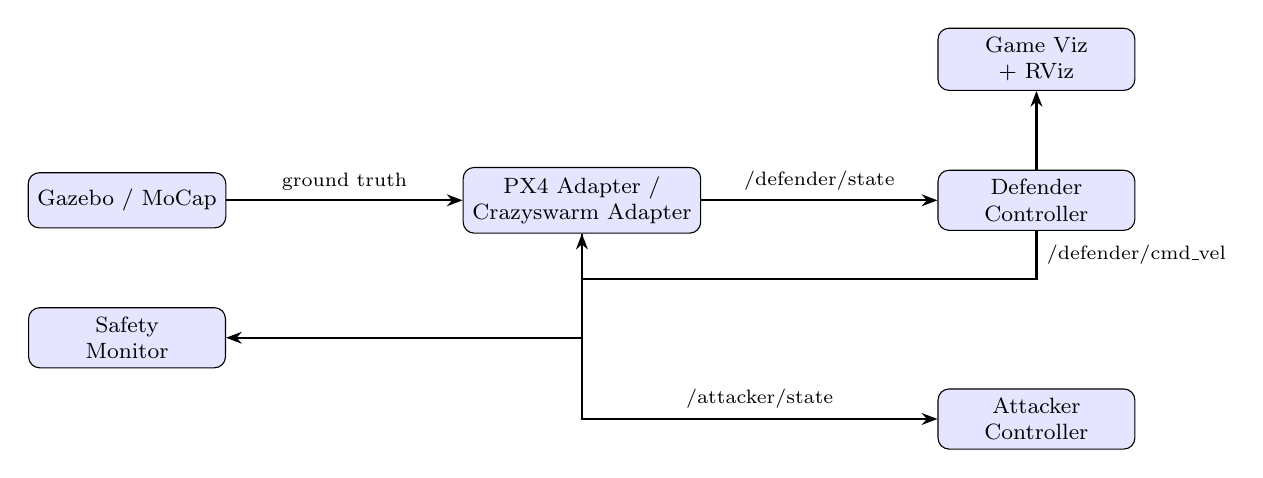
\begin{tikzpicture}[
    node distance=1.5cm and 2.5cm,
    block/.style={rectangle, draw, rounded corners, fill=blue!10, minimum width=2.5cm, minimum height=0.7cm, align=center, font=\footnotesize},
    topic/.style={rectangle, draw, dashed, fill=yellow!10, minimum width=2cm, minimum height=0.5cm, align=center, font=\scriptsize\ttfamily},
    arrow/.style={-{Stealth[length=2mm]}, thick},
]
    \node[block] (gazebo) {Gazebo / MoCap};
    \node[block, right=3cm of gazebo] (adapter) {PX4 Adapter /\\ Crazyswarm Adapter};
    \node[block, right=3cm of adapter] (defender) {Defender\\ Controller};
    \node[block, below=2cm of defender] (attacker) {Attacker\\ Controller};
    \node[block, below=1cm of gazebo] (safety) {Safety\\ Monitor};
    \node[block, above=1cm of defender] (viz) {Game Viz\\ + RViz};

    \draw[arrow] (gazebo) -- node[above, font=\scriptsize] {ground truth} (adapter);
    \draw[arrow] (adapter) -- node[above, font=\scriptsize] {/defender/state} (defender);
    \draw[arrow] (adapter) |- node[near end, above, font=\scriptsize] {/attacker/state} (attacker);
    \draw[arrow] (defender) -- node[right, font=\scriptsize] {/defender/cmd\_vel} ++(0,-1) -| (adapter);
    \draw[arrow] (adapter) |- (safety);
    \draw[arrow] (defender) -- (viz);
\end{tikzpicture}
\end{center}

Key topics:
\begin{itemize}[noitemsep]
    \item \texttt{/defender/state} (\texttt{PoseStamped}) --- defender position from ground truth
    \item \texttt{/attacker/state} (\texttt{PoseStamped}) --- attacker position
    \item \texttt{/defender/cmd\_vel} (\texttt{Twist}) --- velocity command to PX4/Crazyflie
    \item \texttt{/game/status} (\texttt{String}) --- game status and mode, e.g.\ \texttt{DEFENDER\_WINNING | z:tracking h:pid\_pursuit | d\_h=4.32 d\_z=0.12}
    \item \texttt{/safety/emergency} (\texttt{Bool}) --- emergency landing trigger
\end{itemize}

\subsection{Configuration}

All game parameters are defined in \texttt{config/game\_params.yaml}:

\begin{lstlisting}[style=yamlstyle, title=\textbf{Key parameters from game\_params.yaml}]
room:
  x_min: 0.0    x_max: 45.0
  y_min: 0.0    y_max: 25.0
  z_min: 0.0    z_max: 20.0
defender:
  max_speed_horizontal: 6.0    # m/s
  max_speed_vertical: 4.0      # m/s
  k_x: 0.7    k_y: 0.7    k_z: 1.5
attacker:
  max_speed_horizontal: 3.0    # m/s
  max_speed_vertical: 2.0      # m/s
capture:
  d_h: 3.0    # horizontal capture distance (m)
  d_z: 1.0    # vertical capture distance (m)
target_region:
  x_min: 38.0    x_max: 45.0
  y_min: 10.0    y_max: 15.0
obstacles:
  - type: box
    x_min: 15.0    x_max: 20.0
    y_min: 5.0     y_max: 20.0
\end{lstlisting}

Three grid presets are available:

\begin{table}[h]
\centering
\caption{Grid resolution presets.}
\begin{tabular}{lccc}
\toprule
\textbf{Preset} & \textbf{Vertical 2D} & \textbf{Vertical 3D} & \textbf{Horizontal 4D/6D} \\
\midrule
\texttt{dev} & $51 \times 31$ & $24 \times 10 \times 24$ & $21^2 \times 11^2$ \\
\texttt{medium} & $120 \times 50$ & $120 \times 50 \times 120$ & $43^2 \times 6^2$ \\
\texttt{paper} & $240 \times 100$ & $240 \times 100 \times 240$ & $85^2 \times 8^2$ \\
\bottomrule
\end{tabular}
\end{table}


%=============================================================================
\section{Running the Offline Computation}
%=============================================================================

\subsection{Prerequisites}

\begin{lstlisting}[style=bashstyle]
# Install the reach_avoid_game package (editable mode)
cd /workspace/reach_avoid_game
pip install -e ".[dev]"

# Verify installation
python3 -c "import reach_avoid_game; print('OK')"
python3 -c "import hj_reachability; print('hj_reachability OK')"
\end{lstlisting}

\subsection{Computing Value Functions}

The computation must follow the correct dependency order.

\subsubsection{Step 1: Vertical Pipeline}

\begin{lstlisting}[style=bashstyle]
# Compute V_z_inf -> B_z -> Phi_z (with B_z feedback)
python3 /workspace/reach_avoid_game/scripts/compute_vertical.py \
    --preset dev

# Output files:
#   /workspace/data/value_functions/V_z_inf.npz
#   /workspace/data/value_functions/B_z.npz
#   /workspace/data/value_functions/phi_z.npz
#   /workspace/data/value_functions/phi_z_time_slices.npz
\end{lstlisting}

\subsubsection{Step 2: Horizontal Pipeline}

\begin{lstlisting}[style=bashstyle]
# Compute V_h_T -> B_h -> phi_A_reach -> Phi_h (with B_h feedback)
python3 /workspace/reach_avoid_game/scripts/compute_horizontal.py \
    --preset dev

# Optional: include 6D extension
python3 /workspace/reach_avoid_game/scripts/compute_horizontal.py \
    --preset dev --include-6d

# Output files:
#   /workspace/data/value_functions/V_h_T.npz
#   /workspace/data/value_functions/B_h.npz
#   /workspace/data/value_functions/phi_A_reach.npz
#   /workspace/data/value_functions/phi_h.npz
#   /workspace/data/value_functions/V_h_T_6d.npz  (if --include-6d)
\end{lstlisting}

\begin{infobox}
The \texttt{dev} preset takes minutes. The \texttt{medium} preset takes tens of minutes. The \texttt{paper} preset ($\sim$3 hours for $\Phi_h$ alone) requires significant RAM and ideally a GPU.
\end{infobox}

\subsection{Running Numerical Simulations}

\begin{lstlisting}[style=bashstyle]
# Vertical-only simulation (Algorithm 1)
python3 /workspace/reach_avoid_game/scripts/numerical_sim.py \
    --mode vertical --T 10.0

# Combined 3D simulation (Algorithm 1 + Algorithm 2)
python3 /workspace/reach_avoid_game/scripts/numerical_sim.py \
    --mode combined --T 10.0

# Quick sanity check (1 step, verifies value function loading)
python3 /workspace/reach_avoid_game/scripts/numerical_sim.py \
    --mode combined --check-only
\end{lstlisting}

\subsection{Generating Paper Figures}

\begin{lstlisting}[style=bashstyle]
python3 /workspace/reach_avoid_game/scripts/generate_paper_figures.py \
    --output-dir /workspace/data/plots/paper_figures/ \
    --preset dev
\end{lstlisting}

This generates 10 figures corresponding to Figures 4--12 of the paper: $\mathcal{B}_z$ invariant set, $\Phi_z$ slices, vertical 3D view, $\mathcal{B}_h$ invariant set, $\Phi_h$ slices, winning regions, simulation trajectories, and a combined 3D game view.

\subsection{Running Tests}

\begin{lstlisting}[style=bashstyle]
cd /workspace/reach_avoid_game
python3 -m pytest tests/ -v

# 60 tests in reach_avoid_game + 31 in reach_avoid_controller = 91 total
# Covering:
#   - Grid dimensions and value function shapes
#   - Phi_z properties (monotonicity, sign conventions)
#   - B_z non-emptiness and center containment
#   - Control extraction within speed limits
#   - Gradient finite-ness
#   - T_capture from time slices
#   - Winning region partitioning
#   - Value function I/O round-trip
\end{lstlisting}


%=============================================================================
\section{Running the Gazebo Simulation}
%=============================================================================

\subsection{Quick Start (3 Commands)}

The entire simulation runs inside Docker. No local ROS\,2 or Gazebo installation is needed --- only Docker Desktop.

\begin{lstlisting}[style=bashstyle]
# 1. Build the image (first time takes ~20 min, cached afterwards)
docker build -f Dockerfile.sim -t reach-avoid-sim .

# 2. Start the simulation (auto-launches everything)
docker-compose -f docker-compose.sim.yml up

# 3. Verify drones are flying (in a separate terminal, after ~60s)
docker exec -it reach-avoid-sim bash -c \
  'source /opt/ros/humble/setup.bash && \
   source /home/simuser/ws/install/setup.bash && \
   ros2 topic echo /attacker/state --field pose.position --once'
\end{lstlisting}

Expected output after $\sim$60\,s: the attacker's position should be moving from its spawn $(5, 20, 3)$ toward the target $(41.5, 12.5, 10)$.

\begin{warningbox}
On macOS (Apple Silicon or Intel), Gazebo runs headless (no GUI window). The physics simulation, PX4, and all controllers run normally --- you verify via \texttt{ros2 topic echo}. On Linux with a GPU and X11, Gazebo will open a 3D window.
\end{warningbox}

\subsection{What Happens at Startup}

The container's \texttt{CMD} runs \texttt{ros2 launch reach\_avoid\_bringup full\_game.launch.py}, which orchestrates the following startup sequence:

\begin{center}
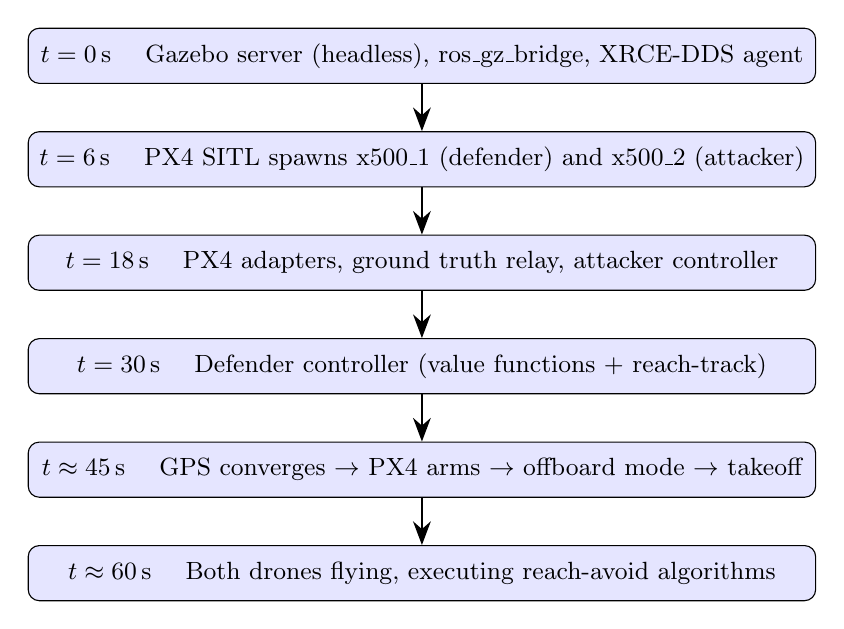
\begin{tikzpicture}[
    node distance=0.6cm,
    block/.style={rectangle, draw, rounded corners, fill=blue!10, minimum width=10cm, minimum height=0.7cm, align=left, font=\small},
]
    \node[block] (t0) {$t = 0$\,s \quad Gazebo server (headless), ros\_gz\_bridge, XRCE-DDS agent};
    \node[block, below=of t0] (t6) {$t = 6$\,s \quad PX4 SITL spawns x500\_1 (defender) and x500\_2 (attacker)};
    \node[block, below=of t6] (t18) {$t = 18$\,s \quad PX4 adapters, ground truth relay, attacker controller};
    \node[block, below=of t18] (t30) {$t = 30$\,s \quad Defender controller (value functions + reach-track)};
    \node[block, below=of t30] (t45) {$t \approx 45$\,s \quad GPS converges $\to$ PX4 arms $\to$ offboard mode $\to$ takeoff};
    \node[block, below=of t45] (t60) {$t \approx 60$\,s \quad Both drones flying, executing reach-avoid algorithms};

    \draw[-{Stealth[length=3mm]}, thick] (t0) -- (t6);
    \draw[-{Stealth[length=3mm]}, thick] (t6) -- (t18);
    \draw[-{Stealth[length=3mm]}, thick] (t18) -- (t30);
    \draw[-{Stealth[length=3mm]}, thick] (t30) -- (t45);
    \draw[-{Stealth[length=3mm]}, thick] (t45) -- (t60);
\end{tikzpicture}
\end{center}

\subsection{Monitoring the Game}

All commands below require the ROS\,2 environment. Use single quotes to avoid shell escaping issues:

\begin{lstlisting}[style=bashstyle]
# Shorthand: define a helper function (optional)
# rexec() { docker exec -it reach-avoid-sim bash -c \
#   "source /opt/ros/humble/setup.bash && \
#    source /home/simuser/ws/install/setup.bash && $1"; }

# --- Check which nodes are running ---
docker exec -it reach-avoid-sim bash -c \
  'source /opt/ros/humble/setup.bash && \
   source /home/simuser/ws/install/setup.bash && \
   ros2 node list'
# Expected: /attacker_controller /defender_controller
#           /ground_truth_relay /kinematic_sim or /px4_adapter_*
#           /game_viz /ros_gz_bridge /world_to_map_tf

# --- Watch attacker position (Ctrl+C to stop) ---
docker exec -it reach-avoid-sim bash -c \
  'source /opt/ros/humble/setup.bash && \
   source /home/simuser/ws/install/setup.bash && \
   ros2 topic echo /attacker/state --field pose.position'

# --- Watch defender position ---
docker exec -it reach-avoid-sim bash -c \
  'source /opt/ros/humble/setup.bash && \
   source /home/simuser/ws/install/setup.bash && \
   ros2 topic echo /defender/state --field pose.position'

# --- Check velocity commands ---
docker exec -it reach-avoid-sim bash -c \
  'source /opt/ros/humble/setup.bash && \
   source /home/simuser/ws/install/setup.bash && \
   ros2 topic echo /defender/cmd_vel --once'

# --- List all active topics ---
docker exec -it reach-avoid-sim bash -c \
  'source /opt/ros/humble/setup.bash && \
   source /home/simuser/ws/install/setup.bash && \
   ros2 topic list'

# --- Check PX4 arm/takeoff status ---
docker logs reach-avoid-sim 2>&1 | grep -iE "armed|takeoff"

# --- Stop the simulation ---
docker-compose -f docker-compose.sim.yml down
\end{lstlisting}

\subsection{Expected Game Behavior}

When the simulation is running correctly:

\begin{enumerate}
    \item \textbf{Attacker} spawns at $(5, 20, 3)$ and uses \textbf{optimal game-theoretic control} by default:
    \begin{itemize}[noitemsep]
        \item Loads $\Phi_h$ and $\Phi_z$ value functions, subscribes to defender state
        \item Extracts bang-bang controls from value function gradients (Eqs.~\ref{eq:attacker-horiz}--\ref{eq:attacker-vert})
        \item Flies at maximum speed: $U_A^h = 3.0$\,m/s horizontal, $U_A^z = 2.0$\,m/s vertical
        \item Actively evades the defender while navigating toward the target region
        \item Obstacle avoidance is implicit in the $\Phi_h$ value function (reach-avoid formulation)
    \end{itemize}
    If launched with \texttt{attacker\_mode:=scripted}, it instead follows 6 waypoints at 1.6\,m/s.

    \item \textbf{Defender} spawns at $(5, 12.5, 3)$ and uses the \textbf{reach-track controller}:
    \begin{itemize}[noitemsep]
        \item Loads precomputed value functions ($\Phi_z$, $V_{z,\infty}$, $\mathcal{B}_z$, $\Phi_h$, $V_{h,T}$, $\mathcal{B}_h$)
        \item Checks if current state is in the defender's \textbf{winning region} ($\Phi \leq 0$)
        \item If in winning region: computes optimal velocity via value function gradients (Algorithm 1 + 2)
        \item If outside winning region: uses \textbf{PID pursuit} --- proportional control driving directly toward the attacker
        \item Velocity clamped to $U_D^h = 6.0$\,m/s horizontal, $U_D^z = 4.0$\,m/s vertical (matching game parameters)
    \end{itemize}

    \item \textbf{Game outcome}: the defender attempts to intercept the attacker before it reaches the target region $x \in [38,45]$, $y \in [10,15]$. Capture occurs when horizontal distance $\leq 3$\,m \textbf{and} vertical distance $\leq 1$\,m (cylindrical capture zone).
\end{enumerate}

\subsection{Attacker Control Modes}

\begin{itemize}[noitemsep]
    \item \texttt{optimal} \textbf{(default)} --- game-theoretic HJ bang-bang control using $\Phi_h$ and $\Phi_z$ gradients. The attacker minimizes the game value function, yielding the optimal evasion strategy from the paper. Requires precomputed value functions and defender state access.
    \item \texttt{scripted} --- follows predefined waypoints toward target at constant speed (1.6\,m/s)
    \item \texttt{keyboard} --- manual control via \texttt{teleop\_twist\_keyboard}
    \item \texttt{switchable} --- start in scripted, switch at runtime via \texttt{/attacker/set\_mode} service
\end{itemize}

To override the default mode in any launch file:
\begin{lstlisting}[style=bashstyle]
ros2 launch reach_avoid_bringup full_game.launch.py attacker_mode:=scripted
\end{lstlisting}

\subsection{Architecture Details}

\subsubsection{Docker Image}

The \texttt{Dockerfile.sim} builds on Ubuntu 22.04 with:
\begin{itemize}[noitemsep]
    \item ROS\,2 Humble Desktop + Gazebo Harmonic + ros\_gz bridge
    \item PX4 Autopilot compiled for SITL with \texttt{gz\_x500} quadrotor model
    \item micro-XRCE-DDS-Agent (PX4 $\leftrightarrow$ ROS\,2 bridge)
    \item \texttt{px4\_msgs} and \texttt{px4\_ros\_com} for PX4 message types
    \item The full \texttt{reach\_avoid\_ws} workspace, pre-built with \texttt{colcon build}
    \item Value functions and game parameters copied from host
\end{itemize}

\subsubsection{Gazebo World}

The SDF world (\texttt{reach\_avoid\_arena.sdf}) defines:
\begin{itemize}[noitemsep]
    \item $45 \times 25 \times 20$\,m room with four walls (matching \texttt{game\_params.yaml})
    \item Red obstacle: $x \in [15,20]$, $y \in [5,20]$ (center $(17.5, 12.5, 10)$, size $5 \times 15 \times 20$\,m)
    \item Green target region: $x \in [38,45]$, $y \in [10,15]$ (center $(41.5, 12.5, 10)$, size $7 \times 5 \times 20$\,m)
    \item Spherical coordinates (Zurich, 47.40\textdegree N, 8.55\textdegree E) for GPS sensor
    \item NavSat system plugin for GPS simulation
    \item DART physics at 1\,kHz
\end{itemize}

\subsubsection{PX4 SITL Configuration}

Each PX4 instance runs with these parameters (set via \texttt{PX4\_PARAM\_*} environment variables):

\begin{table}[h]
\centering
\small
\caption{PX4 SITL parameter configuration.}
\begin{tabular}{llp{6cm}}
\toprule
\textbf{Parameter} & \textbf{Value} & \textbf{Purpose} \\
\midrule
\texttt{EKF2\_GPS\_CTRL} & 7 & GPS fusion (position + velocity + altitude) \\
\texttt{EKF2\_MAG\_TYPE} & 1 & Automatic magnetometer fusion \\
\texttt{EKF2\_MAG\_CHECK} & 0 & Disable mag consistency check \\
\texttt{COM\_ARM\_WO\_GPS} & 1 & Allow arming before GPS lock \\
\texttt{CBRK\_SUPPLY\_CHK} & 894281 & Bypass power supply check \\
\texttt{CBRK\_FLIGHTTERM} & 121212 & Bypass flight termination \\
\texttt{COM\_DISARM\_PRFLT} & $-1$ & Disable auto preflight disarm \\
\texttt{FD\_FAIL\_P/R} & 0 & Disable pitch/roll failure detection \\
\texttt{COM\_IMB\_PROP\_ACT} & 0 & Disable propeller imbalance action \\
\bottomrule
\end{tabular}
\end{table}

\subsubsection{Ground Truth Relay}

The ground truth relay node bridges PX4 local position to game coordinates:

\begin{itemize}[noitemsep]
    \item Subscribes to PX4's \texttt{VehicleLocalPosition} via \texttt{px4\_msgs} (50\,Hz)
    \item Converts NED (North-East-Down) to ENU (East-North-Up) by swapping $x \leftrightarrow y$ and negating $z$
    \item Adds spawn position offsets: defender $(5, 12.5, 3)$, attacker $(5, 20, 3)$
    \item Publishes to \texttt{/defender/state} and \texttt{/attacker/state} as \texttt{PoseStamped}
\end{itemize}

\subsubsection{PX4 Adapter}

The PX4 adapter translates velocity commands to PX4 offboard control:

\begin{itemize}[noitemsep]
    \item Subscribes to \texttt{/defender/cmd\_vel} (or \texttt{/attacker/cmd\_vel})
    \item Clamps velocities to $U_D^h = 6.0$\,m/s horizontal, $U_D^z = 4.0$\,m/s vertical (matching game parameters)
    \item Converts ENU to NED and publishes \texttt{TrajectorySetpoint} + \texttt{OffboardControlMode}
    \item Auto-engages offboard mode and force-arms PX4 after GPS convergence ($\sim$15\,s)
\end{itemize}

\subsection{Kinematic Simulation Mode (No PX4)}

For faster iteration or environments where PX4 SITL is problematic, a lightweight kinematic simulator is available:

\begin{lstlisting}[style=bashstyle]
# In docker-compose.sim.yml, change the command to:
command: ros2 launch reach_avoid_bringup kinematic_game.launch.py

# Or run directly inside the container:
ros2 launch reach_avoid_bringup kinematic_game.launch.py
\end{lstlisting}

This mode replaces Gazebo + PX4 with simple velocity integration ($\mathbf{x}_{t+1} = \mathbf{x}_t + \mathbf{v} \cdot \Delta t$). The reach-avoid controllers are identical --- only the physics layer changes. Startup is instant (no GPS convergence wait).


%=============================================================================
\section{Running on Real Drones}
%=============================================================================

\begin{dangerbox}
Hardware deployment involves real flying robots. Always have a safety pilot ready. Always test with conservative speed limits first. The safety monitor will trigger emergency landing on any violation, but human oversight is essential.
\end{dangerbox}

\subsection{Hardware Requirements}

\begin{table}[h]
\centering
\caption{Required hardware components.}
\begin{tabular}{lp{8cm}}
\toprule
\textbf{Component} & \textbf{Details} \\
\midrule
Crazyflie 2.1 (x2) & One defender, one attacker. Must have unique radio addresses. \\
Crazyradio PA (x1) & USB radio dongle for communicating with Crazyflies. \\
Motion capture system & OptiTrack, Vicon, or similar. Must publish pose at $\geq$100\,Hz. \\
Ground station PC & Ubuntu 22.04, ROS\,2 Humble, Crazyswarm2 installed. \\
Flying arena & Minimum $4 \times 4 \times 3$\,m clear space with safety nets. \\
\bottomrule
\end{tabular}
\end{table}

\subsection{Software Setup}

\begin{lstlisting}[style=bashstyle]
# 1. Install ROS 2 Humble (if not already installed)
sudo apt install ros-humble-desktop

# 2. Install Crazyswarm2
mkdir -p ~/crazyswarm2_ws/src
cd ~/crazyswarm2_ws/src
git clone https://github.com/IMRCLab/crazyswarm2
cd ..
colcon build --symlink-install
source install/setup.bash

# 3. Build the reach_avoid_ws workspace
cd /workspace/reach_avoid_ws
source /opt/ros/humble/setup.bash
colcon build --symlink-install
source install/setup.bash

# 4. Install the offline computation package
cd /workspace/reach_avoid_game
pip install -e .

# 5. Compute value functions (use medium or paper preset for real flights)
python3 scripts/compute_vertical.py --preset medium
python3 scripts/compute_horizontal.py --preset medium
\end{lstlisting}

\subsection{Crazyflie Configuration}

Edit \texttt{reach\_avoid\_bringup/config/hardware\_params.yaml}:

\begin{lstlisting}[style=yamlstyle]
crazyswarm_adapter:
  ros__parameters:
    defender_uri: "radio://0/80/2M/E7E7E7E701"
    attacker_uri: "radio://0/80/2M/E7E7E7E702"
    mocap_topic: "/mocap/rigid_bodies"
    takeoff_height: 1.0
    cmd_rate: 20.0
\end{lstlisting}

Change the URIs to match your Crazyflie radio addresses. The motion capture topic must match your MoCap system's ROS\,2 output.

\subsection{Pre-Flight Checklist}

\begin{enumerate}
    \item Charge both Crazyflie batteries fully.
    \item Verify motion capture tracking for both drones (all rigid body markers visible).
    \item Place drones at known starting positions within the arena.
    \item Verify radio link: \texttt{cfclient} should show both drones.
    \item Confirm value function files exist in \texttt{/workspace/data/value\_functions/}.
    \item Clear the arena of people and obstacles not part of the experiment.
    \item Brief the safety pilot on emergency procedures.
\end{enumerate}

\subsection{Launch Sequence}

\begin{lstlisting}[style=bashstyle]
# Terminal 1: Source workspace
source /workspace/reach_avoid_ws/install/setup.bash

# Terminal 2: Launch the hardware game
ros2 launch reach_avoid_bringup hardware.launch.py \
    attacker_mode:=optimal \
    value_function_dir:=/workspace/data/value_functions/ \
    defender_uri:=radio://0/80/2M/E7E7E7E701 \
    attacker_uri:=radio://0/80/2M/E7E7E7E702 \
    use_rviz:=true

# Terminal 3: Arm the safety monitor
ros2 service call /safety/arm std_srvs/srv/Trigger

# Terminal 4: Command takeoff
ros2 service call /hw/takeoff std_srvs/srv/Trigger

# The defender controller will automatically begin tracking the attacker
# once both drone states are being received.

# Emergency landing (any terminal):
ros2 service call /hw/land std_srvs/srv/Trigger
\end{lstlisting}

\subsection{Safety Monitor}

The safety monitor node (\texttt{reach\_avoid\_hw/safety\_monitor\_node.py}) runs at 50\,Hz and checks:

\begin{table}[h]
\centering
\caption{Safety checks and their parameters.}
\begin{tabular}{lll}
\toprule
\textbf{Check} & \textbf{Condition} & \textbf{Default} \\
\midrule
Geofence & Position within room bounds $\pm$ margin & 0.5\,m margin \\
Altitude floor & $z > z_\text{min}$ & 0.3\,m \\
Altitude ceiling & $z < z_\text{max} - \text{margin}$ & 0.5\,m margin \\
Defender speed & $\|v\| < U_D \times 1.1$ & 6.6\,m/s \\
Attacker speed & $\|v\| < U_A \times 1.1$ & 3.3\,m/s \\
Inter-drone distance & $\|p_D - p_A\| > d_\text{min}$ & 0.5\,m \\
State watchdog & State received within timeout & 1.0\,s \\
\bottomrule
\end{tabular}
\end{table}

\textbf{Fail-safe behavior:} The safety monitor defaults to emergency landing on:
\begin{itemize}[noitemsep]
    \item Any safety violation
    \item State data timeout (communication loss)
    \item Any internal error (exception during safety check)
\end{itemize}

The emergency state \textbf{latches} --- once triggered, the monitor stays in emergency until manually rearmed via the \texttt{/safety/arm} service.

\subsection{Crazyswarm2 Adapter}

The adapter node bridges the reach-track controller to the Crazyflie hardware:

\begin{itemize}
    \item Subscribes to \texttt{/defender/cmd\_vel} (Twist) from the defender controller.
    \item Forwards velocity commands to the Crazyflie via \texttt{cmdVelocityWorld}.
    \item Reads motion capture poses from \texttt{/mocap/defender} and \texttt{/mocap/attacker}.
    \item Publishes drone states (\texttt{/defender/state}, \texttt{/attacker/state}) and velocity estimates.
    \item Provides takeoff (\texttt{/hw/takeoff}) and landing (\texttt{/hw/land}) services.
\end{itemize}

Velocity estimation is done via finite differences on motion capture position data. For more accurate velocity, consider using the Crazyflie's onboard state estimator.

\subsection{Tuning for Real Hardware}

\begin{warningbox}
The value functions computed with the paper's speed parameters ($U_D^h = 6$\,m/s) may be too aggressive for indoor Crazyflie flights. Recommended adjustments for initial testing:
\begin{itemize}[noitemsep]
    \item Reduce \texttt{max\_speed\_horizontal} to 1.0--2.0\,m/s
    \item Reduce \texttt{max\_speed\_vertical} to 0.5--1.0\,m/s
    \item Increase \texttt{min\_inter\_drone\_distance} to 1.0\,m
    \item Recompute value functions with the adjusted parameters
\end{itemize}
\end{warningbox}

The proportional gains ($k_x$, $k_y$, $k_z$) model the Crazyflie's velocity response. Measure the actual step response of your drone and adjust these gains to match. A gain that is too high will cause the value function to overestimate the drone's agility; too low will make it too conservative.


%=============================================================================
\section{End-to-End Simulation Results}
%=============================================================================

The game has been validated using a standalone kinematic simulation (\texttt{tests/integration/test\_kinematic\_game.py}) that replicates the full ROS\,2 kinematic game without requiring ROS\,2 or Gazebo. The simulation uses:

\begin{itemize}[noitemsep]
    \item \textbf{Kinematic simulator}: simple velocity integration with arena bounds clamping (matching \texttt{kinematic\_sim\_node.py})
    \item \textbf{Defender}: double integrator dynamics with reach-track control ($\dot{v} = K(u - v)$, gains from \texttt{game\_params.yaml})
    \item \textbf{Attacker}: single integrator with either scripted waypoint following (1.6\,m/s) or optimal bang-bang control (3.0\,m/s)
    \item \textbf{Capture condition}: horizontal distance $\leq 3$\,m and vertical distance $\leq 1$\,m
\end{itemize}

\subsubsection{Scripted Attacker Scenarios}

\begin{table}[h]
\centering
\caption{Defender vs.\ scripted attacker (all scenarios captured successfully).}
\begin{tabular}{lccl}
\toprule
\textbf{Scenario} & \textbf{Capture Time} & \textbf{Initial Separation} & \textbf{Notes} \\
\midrule
Paper initial conditions & 1.4\,s & 7.5\,m & D at $(5, 12.5, 3)$, A at $(5, 20, 3)$ \\
Attacker ahead, straight line & 4.6\,s & 15.0\,m & A heading directly to target \\
Attacker around obstacle & 1.8\,s & 7.0\,m & A navigating below obstacle \\
Altitude difference & 3.5\,s & 12.0\,m ($z$) & D at $z{=}3$, A at $z{=}15$ \\
\bottomrule
\end{tabular}
\end{table}

\subsubsection{Optimal Attacker Scenario}

When the attacker uses game-theoretic optimal control, the game becomes significantly more competitive. The attacker applies bang-bang controls from $\Phi_h$ and $\Phi_z$ gradients, flying at maximum speed (3.0\,m/s horizontal, 2.0\,m/s vertical) and actively evading the defender:

\begin{table}[h]
\centering
\caption{Defender vs.\ optimal attacker.}
\begin{tabular}{lccl}
\toprule
\textbf{Scenario} & \textbf{Capture Time} & \textbf{Initial Separation} & \textbf{Notes} \\
\midrule
Optimal attacker vs.\ optimal defender & 4.2\,s & 7.5\,m & D at $(5, 12.5, 3)$, A at $(5, 20, 3)$ \\
\bottomrule
\end{tabular}
\end{table}

\subsubsection{Optimal Attacker Behavior Validation}

The test suite includes dedicated behavioral assertions that verify the optimal controller works correctly:

\begin{table}[h]
\centering
\caption{Optimal attacker behavior validation results.}
\begin{tabular}{lll}
\toprule
\textbf{Check} & \textbf{Expected} & \textbf{Measured} \\
\midrule
Average horizontal speed & $> 1.0$\,m/s & 4.24\,m/s \\
Commands at near-max speed ($\geq U_A^h$) & $> 50\%$ & 100\% \\
X-axis progress in 5\,s & $> 3.0$\,m & 12.3\,m \\
Altitude after 5\,s (from $z = 3$) & $> 4.0$\,m & 10.0\,m \\
Path divergence from scripted (5\,s) & $> 1.0$\,m & 13.3\,m \\
Evasion reaction to defender position & Y-command differs & $\Delta = 6.0$\,m/s \\
\bottomrule
\end{tabular}
\end{table}

Key findings:
\begin{itemize}[noitemsep]
    \item The optimal attacker flies at \textbf{bang-bang speed} (100\% of commands at $U_A^h = 3.0$\,m/s per axis, yielding $\sim$4.24\,m/s diagonal).
    \item It makes rapid progress toward the target (\textbf{12.3\,m} of x-progress in 5\,s).
    \item Its path \textbf{diverges by 13.3\,m} from the scripted waypoint path after 5\,s --- it is using a fundamentally different, game-theoretically optimal trajectory.
    \item When the defender changes position (above vs.\ below), the attacker's y-command reverses by \textbf{6.0\,m/s} --- a full bang-bang sign flip, demonstrating active evasion.
\end{itemize}

\begin{lstlisting}[style=bashstyle, title=\textbf{Running the standalone simulation}]
# No ROS2 needed --- runs in pure Python with value functions
cd /workspace
python3 tests/integration/test_kinematic_game.py
\end{lstlisting}


%=============================================================================
\section{Troubleshooting}
%=============================================================================

\begin{description}[style=nextline, leftmargin=0.5cm]
    \item[\texttt{Phi\_z} is all positive (no winning region)]
    On coarse grids (dev preset), the invariant capture set $\mathcal{B}_z$ may be very small, causing $\Phi_z$ to remain positive everywhere. Use the \texttt{medium} or \texttt{paper} preset for meaningful results.

    \item[\texttt{T\_capture} returns infinity]
    Same root cause as above. The time slices never reach $\leq 0$ on coarse grids because $\mathcal{B}_z$ is too small as a target set.

    \item[Docker build fails: package not found]
    ROS\,2 packages (\texttt{python3-colcon-common-extensions}, etc.) must be installed \textbf{after} the ROS\,2 apt repository is added. The Dockerfile adds repos first, then installs all packages in a single \texttt{apt-get install}.

    \item[\texttt{nvidia} runtime error on macOS]
    macOS has no NVIDIA GPU. The \texttt{docker-compose.sim.yml} has the \texttt{runtime: nvidia} and GPU sections commented out. Gazebo runs headless (\texttt{-s} server mode) without a display.

    \item[PX4 ``Arming denied: system health failures'']
    PX4 requires GPS lock before arming. The SDF world must include \texttt{<spherical\_coordinates>} (with valid lat/lon) and the \texttt{gz-sim-navsat-system} plugin. GPS convergence takes $\sim$15--30\,s after drone spawn. The adapter uses force-arm (\texttt{param2=21196}) to bypass remaining preflight checks.

    \item[PX4 \texttt{xy\_valid: false}]
    EKF2 has no horizontal position. Causes: (1)~missing \texttt{<spherical\_coordinates>} in SDF; (2)~missing NavSat system plugin; (3)~\texttt{EKF2\_GPS\_CTRL=0} (GPS fusion disabled). Set \texttt{EKF2\_GPS\_CTRL=7} and add both SDF elements.

    \item[PX4 compass fault / imbalanced propeller]
    Common in headless SITL, especially with aggressive velocity commands. Mitigations: set \texttt{EKF2\_MAG\_CHECK=0}, \texttt{COM\_IMB\_PROP\_ACT=0}, \texttt{CBRK\_FLIGHTTERM=121212}. Reduce velocity clamp in the PX4 adapter (default: 1.5\,m/s horizontal, 1.0\,m/s vertical).

    \item[\texttt{numpy.\_core} ModuleNotFoundError]
    Value function \texttt{.npz} files were saved with numpy 2.x but the container has numpy 1.x. The \texttt{value\_function\_loader.py} catches this error and falls back to empty params (the controller uses hardcoded defaults). Not a critical error.

    \item[\texttt{/defender/state} or \texttt{/attacker/state} hangs (no data)]
    The ground truth relay is not receiving PX4 position data. Check: (1)~\texttt{px4\_msgs} is importable --- the Dockerfile sets \texttt{PYTHONPATH} to include the px4\_ros\_ws install; (2)~PX4 local position topic is publishing: \texttt{ros2 topic hz /defender/fmu/out/vehicle\_local\_position\_v1}; (3)~the node is running: \texttt{ros2 node list} should show \texttt{/ground\_truth\_relay}.

    \item[Defender flies away from attacker instead of toward it]
    On coarse grids (dev preset), the 6D value function $\Phi_h$ may not resolve the capture set --- $\Phi_h > 0$ everywhere, and gradients point in arbitrary directions. \textbf{Solution:} The controller checks if the state is in the winning region ($\Phi \leq 0$) before using HJ optimal control. Outside the winning region, it falls back to PID pursuit. This was fixed in v0.2.0. If you still see wrong-direction behavior, verify value functions were recomputed after the update.

    \item[Defender flies out of bounds / unstable flight]
    The reach-track controller outputs maximum velocity ($U_D^h = 6$\,m/s), which may cause motor saturation in PX4's x500 model. The PX4 adapter now clamps velocities to the game parameters (6.0\,m/s horizontal, 4.0\,m/s vertical). For real hardware or if PX4 is unstable, reduce these values in the PX4 adapter's \texttt{max\_h} / \texttt{max\_v} constants or use the kinematic simulation mode.

    \item[Drones arm but immediately disarm]
    PX4's auto preflight disarm triggers if no takeoff occurs within the timeout. Set \texttt{COM\_DISARM\_PRFLT=$-1$} to disable. Also ensure offboard mode is engaged \textbf{before} arming --- the adapter sends 40 setpoints, engages offboard, waits 20 more setpoints, then arms.
\end{description}


%=============================================================================
\section{References}
%=============================================================================

\begin{enumerate}
    \item M.~Bui, S.~Monckton, and M.~Chen, ``Reach-Avoid Differential Game with Reachability Analysis for UAVs --- A Decomposition Approach,'' \textit{arXiv preprint arXiv:2512.22793}, Dec.~2025.

    \item \texttt{hj\_reachability}: \url{https://github.com/StanfordASL/hj_reachability} --- JAX-based Hamilton-Jacobi reachability library (v0.7.0). Used as the numerical backend for the OptimizedDP-compatible solver.

    \item M.~Bui, A.~Brandao~Araujo, and M.~Chen, ``OptimizedDP: An Efficient, User-friendly Library For Optimal Control and Dynamic Programming,'' \textit{arXiv preprint arXiv:2204.05520}, 2022. \url{https://github.com/SFU-MARS/optimized_dp}. The API design for our solver layer follows this library's conventions.

    \item PX4 Autopilot: \url{https://github.com/PX4/PX4-Autopilot} --- Open-source flight controller.

    \item Crazyswarm2: \url{https://github.com/IMRCLab/crazyswarm2} --- ROS\,2 driver for Crazyflie drones.

    \item Gazebo: \url{https://gazebosim.org/} --- Robotics simulation platform (Harmonic release).
\end{enumerate}

\end{document}
